\section{Diseño}

Para el modelado de este proyecto se buscó utilizar prácticas recomendadas y algunos de los patrones vistos con el fin de obtener un modelo cerrado para la modificación pero abierto para la extensión, minimizar la repetición de código, crear buenas abstracciones y permitir variaciones de comportamiento eficientes en tiempo de ejecución. Es importante recalcar que, tal como se explicó en los comentarios de la experiencia con $Scrum$, el modelado no siempre precedió a la implementación, sino que ambos procesos se vieron intercalados y retroalimentados a medida que se avanzaban con distintas $user\ stories$ y se realizaban puestas en común entre el grupo. En esta sección presentamos la visión final del diseño con aquellas soluciones que concluímos eran las más adecuadas, aunque se incluyen comentarios respecto a qué ideas se descartaron o modificaron cuando resulte relevante el contraste.

\subsection{Idea general}

En esta primera etapa del desarrollo, la HOP regula los cultivos de dos maneras: mediante un monitoreo pautado por un plan maestro y por medio de suministros arbitrarios programados en un plan de suministros. Esta interacción con el mundo real está dada, en principio, por dos vías: la recepción de datos mediante sensores y la aplicación de suministros mediante actuadores. Existe una tercera vía de comunicación con el exterior, la cual importa para la toma de decisiones, e involucra envío de mensajes a terceros (se descuenta la interacción por pantalla para mostrar información general).\\
\indent En el caso del plan maestro, éste define para una serie de estadíos fenológicos el estado de suelo deseado (humedad, temperatura, ph). El de suministros, en cambio, debe proveer la programación de insumos para una jornada, lo que incluye una lista de actuadores por cada hora del día y una medida a suministrar para cada uno. Tanto el monitoreo como el suministro arbitrario está a su vez regulado por supervisores que, según su tipo, pedirán información a sensores y en base a esto desencadenarán o no una cadena de responsabilidades hasta que se llegue a una decisión respecto de si suministrar el insumo adecuado o no.

\subsection{Plan Maestro - Estados y Magnitudes}

Antes de comenzar a hablar de las componentes más ricas del diseño es necesario detallar brevemente la parte más sencilla del mismo, que tiene que ver con la representación de parte de la información que se necesita conocer o decir sobre la realidad. Por un lado, se cuenta con la clase concreta \textsl{Medida}, que poseee como colaboradores internos una cantidad y una constante que da cuenta de la unidad correspondiente. Esto permite modelar tanto la información (medición) que se obtiene de los sensores así como también cuantificar el suministro de insumos (esto permitirá representar distintas magnitudes según se definan nuevas unidades, tanto para la incorporación de otros sensores como para el suministro de nuevos insumos). Luego, \textsl{EstadoSuelo} se compone de tres datos: medidas de temperatura, ph y humedad. Algo parecido sucede con \textsl{EstadoMeteorológico}, que a diferencia de la primera - que se utiliza para administrar el suelo en estadíos fenológicos - se utiliza para modelar el clima. Finalmente, la clase \textsl{Etapa} sólo se utiliza para encapsular nombres de estadíos fenológicos, que se definen de manera global para toda la HOP.\\
\indent A partir de estas representaciones básicas entra en juego la clase contenedora \textsl{PlanMaestro}, que posee como variable de instancia un \textsl{Diccionario}\verb|<|\textsl{Etapa, EstadoSuelo}\verb|>| mediante el cual permite definir las etapas fenológicas a monitorear y los valores esperados del estado del suelo. Notar que este modelo permite agregar estados o modificar los existentes dinámicamente (aunque esto último tendrá un impacto como se verá luego).\\
\indent En una los albores de la planificación y posterior modelado, el Plan Maestro tenía más responsabilidades que simplemente dictar cuál es el estado ideal de los cultivos: debía determinar también acciones a llevar adelante, información del estado, comunicación con la central meteorológica, etc. Esta idea desembocaba en un objeto que centralizaban gran parte de la lógica de resolución del problema y, claramente, tenían varios ejes de cambio y mucho acoplamiento, lo cual se fue decantando de manera natural a medida que se iteraba sobre el modelo con nuevas ideas y patrones de diseño.

\subsection{Plan de Suministros - Actuadores}

En primera medida debemos hablar de la clase \textsl{Suministro}, que cuenta con un nombre y una cantidad mínima (de tipo \textsl{Medida}) y representa algún insumo a administrar por la HOP. Esto queda determinado por el nombre con que se cree el objeto de esta clase, mientras que la cantidad mínima representa la medida absoluta por defecto de ese insumo que tendrá algún impacto en el entorno (luego es utilizada como la medida a administrar en los monitoreos). Dado que éstos productos se administran a los cultivos mediante actuadores, existe también la abstracción \textsl{Actuador}, cuyas instancias conocen un nombre (que da cuenta de la acción que realiza el actuador) y el suministro que aplican.\\
\indent En los primeros esbozos de diseño, el plan de suministros también fue concebido como una megaentidad con múltiples responsabilidades. Existía la noción sobre el monitoreo del estado del suelo, pero en ese entonces se pensaba en utilizar al plan como un ente de consulta al cual preguntarle para cierta medición de alguna magnitud y dependiendo del estado o la hora qué había que hacer. A medida que avanzó el proyecto, y que se abordaron otras historias, se fue viendo cómo esas responsabilidades recaían en otras componentes de la HOP, dejando a la clase \textsl{PlanSuministros} con la única tarea de definir la programación de insumos para un período de 24 horas. Cuenta con dos variables de instancia de tipo lista: una contiene 24 listas de actuadores, que representan aquellos programados a accionarse en cada una de las 24 horas del día; la otra, un diccionario de medidas para cada actuador único en la programación. Vale notar que aquí la idea es que se permita suministrar una cantidad arbitraria, mientras que cuando se quiere reestablecer el estado deseado en el monitoreo se utilizan medidas mínimas (ver próxima sección).

\begin{figure}[h!]
  \centering
  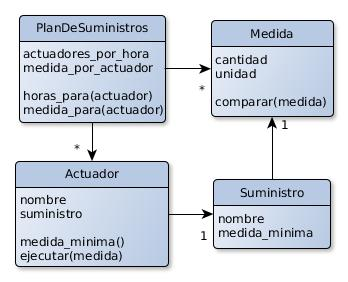
\includegraphics[width=0.5\textwidth]{./imagenes/clases4.jpg}
  \caption{Diagrama de Clases en relación al Plan de Suministros}
  \label{fig:clases4}
\end{figure}


\subsection{Monitoreo y regulación mediante Supervisores}

Otra de las componentes sencillas que falta nombrar son los sensores, representados en el modelo mediante la interface \textsl{InterfazSensor} cuya única operación importante es la de medir. La idea detrás de esta concepción es que distintas claes implementen esta interfaz para distintos sensores físicos, y que con alguna lógica devuelvan un objeto de la clase \textsl{Medida}. De esta manera se pueden tener sensores de las magnitudes que interesan al modelo actual de la huerta (tempratura, humedad, ph) pero además también tiempo, lo cual como se verá adelante es sumamente poderoso para unificar el monitoreo y la administración de insumos planificada en un mismo modelo.\\
\indent Por otro lado, se ideó la clase concreta \textsl{Suministrador}, cuyo propósito es servir como una capa más de lógica entre el actuador y su interacción con el ambiente. Los objetos de esta clase conocen un actuador, una medida arbitraria y un conjunto de responsables (Ver Cadena de Responsabilidad). Posee un único método, $alertar$, que desencadena una cadena de responsabilidades que se utiliza para consultar vinculantemente si se debe suministrar la cantidad determinada a través del actuador conocido.\\ 
\indent El concepto que unifica gran parte de estas ideas, y que funciona como mediador entre la realidad y la lógica de la HOP, es modelado por la clase \textsl{Supervisor}. El objetivo de esta clase es que sus instancias se encarguen de monitorear algún sensor, pidiendole una medición cada cierta cantidad de tiempo (ver Observable). La lógica para analizar esa medición se encontrará en alguna de las clases que heredan de Supervisor, y deben implementar los métodos abstractos $falta$ y $sobra$. Esto permite extender el comportamiento de los supervisores, teniendo por ejemplo la clase \textsl{SupervisorMinMax} para determinar un intervalo óptimo deseado, o la clase \textsl{SupervisorHora}, que posee una colección de enteros entre los que se puede buscar si existe la medición dada. En caso de que alguno de estos métodos devuelva verdadero, el supervisor accionará el método $alertar$ de alguno de sus suministradores, de exceso según si sobra o defecto según si falta.\\
\indent En la Figura~\ref{fig:clases_sup} puede verse el diagrama de clases que exhibe la relación entre parte de las distintas entidades involucradas en este proceso de monitoreo / regulación.

\begin{figure}[h!]
  \centering
  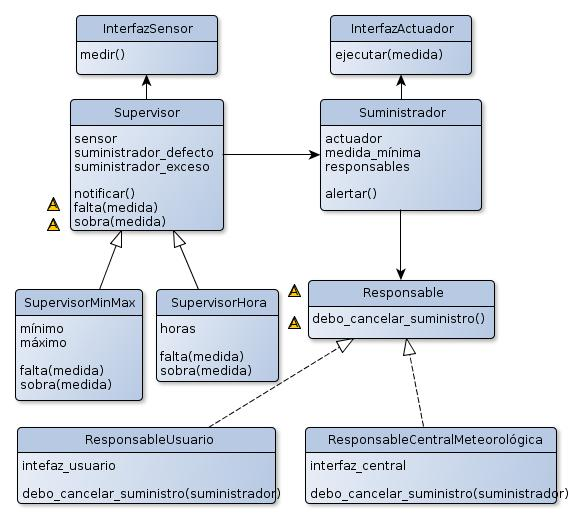
\includegraphics[width=0.8\textwidth]{./imagenes/clases2.jpg}
  \caption{Diagrama de Clases en relación al Supervisor}
  \label{fig:clases_sup}
\end{figure}

\subsection{Cadena de responsabilidades}

Otra característica interesante incorporada al modelo a raíz de la necesidad de interactuar con la central meteorológica fue la de cadena de responsabilidades. En esencia, lo que se trata con esto es de configurar, para cada suministrador, un conjunto de responsables que responden a la pregunta de si debe cancelar la administración de un suministro (en caso de que su supervisor lo hubiera alertado por falta o sobra). Esta lógica está incorporada en el método $alertar$, e itera sobre la colección de responsables abortando sólo si la respuesta es afirmativa para la cancelación. Esto permite que para distintos suministradores (según se utilicen para insumos de monitoreo o programados) exista una consulta vinculante al usuario, a la central meteorológica o eventualmente a otros entes terceros que puedan aportar alguna decisión. Para cada suministrador se puede ordenar la colección de distinta forma, cambiando así dinámicamente las prioridades que se asignan a cada integrante de la cadena. Como se muestra en la Figura~\ref{fig:clases_resp}, la clase \textsl{Responsable} es una interfaz cuyo método $debe_cancelar_suministro$ debe ser implementado por las clases concretas que la realicen. De esta manera, contamos por ejemplo con un \textsl{ResponsableUsuario} o \textsl{ResponsableCentralMeteorológica} que, según distintos colaboradores internos (que por lo general serán interfaces con las que hablan para indagar información según suministro) saben contribuir o dictar una decisión. 

\begin{figure}[h!]
  \centering
  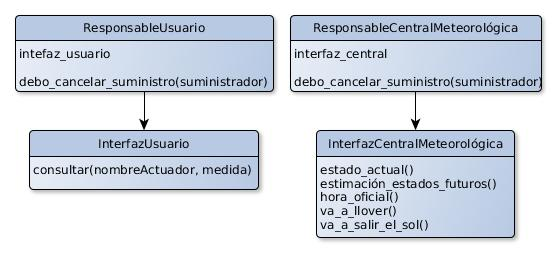
\includegraphics[width=0.6\textwidth]{./imagenes/clases.jpg}
  \caption{Diagrama de Clases en relación a Responsable}
  \label{fig:clases_resp}
\end{figure}

\subsection{Observables}

Un factor fundamental de este modelo es el paso del tiempo, el cual está intimamente ligado al monitoreo de la HOP y la ejecución de suministros programados. Una vez que concluimos en utilizar el diseño mostrado más arriba nos encontramos con la dificultad de determinar quién tomaría el rol de avisar a los distintos supervisores que debían supervisar. La solución se formuló utilizando el patrón $observer$. Si bien al día de la fecha el tiempo está simulado mediante el llamado manual a una función, sí existe una abstracción que es la que posee este método y que es \textsl{Reloj} que hereda de la clase abstracta Observable. El patrón utilizado aquí permite que distintos objetos se suscriban a una instancia de la clase y que luego, en el caso de \textsl{Reloj} mediante el método $tick$, sean notificados. Cada observado debe implementar este método ($notificar$), y el uso que se le dio en este modelo es que los supervisores, al momento de su creación, se suscribieran a una instancia de Reloj; luego con cada $tick$ son notificados y es su implementación de este método la que accióna el pedido de medición al sensor y demás, como se explicó antes. 

\begin{figure}[h!]
  \centering
  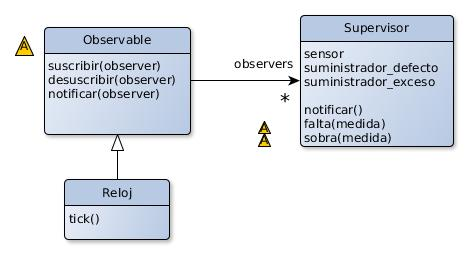
\includegraphics[width=0.6\textwidth]{./imagenes/clases3.jpg}
  \caption{Diagrama de Clases con patrón observer}
  \label{fig:clases_obs}
\end{figure}

\subsection{Coordinador}
Los parámetros utilizados para decidir si una medición provoca o no una alerta van a variar según la etapa en la que se encuentre el cultivo. Esto provocará que los supervisores que se encargan de tomar esas decisiones tengan que cambiar su funcionamiento. Sin embargo, el resto de los objetos no deben verse afectados en absoluto. Por esta razón, decidimos agregar al diseño un coordinador, encargado de mantener la información necesaria para modificar los supervisores que se encuentran operando. Este coordinador mantiene la información del Plan Maestro y los distintos Planes de Suministro por etapa, así como los actuadores y acciones disponibles, de manera tal de poder combinarlas correctamente cada vez que cambie la etapa fenológica.

\clearpage 

\subsection{Situaciones Ejemplo}

A continuación se exhiben un diagrama de objetos y  algunos diagramas de secuencia que muestran distintas situaciones de monitoreo y regulación por parte de la HOP, incluida la cadena de responsabilidades y la interacción con el reloj. El uso de estos ejemplos tiene relevancia ya que exhibe, a nuestro criterio, una conjunción de los aspectos de diseño más interesantes. 

\begin{figure}[h!]
  \centering
  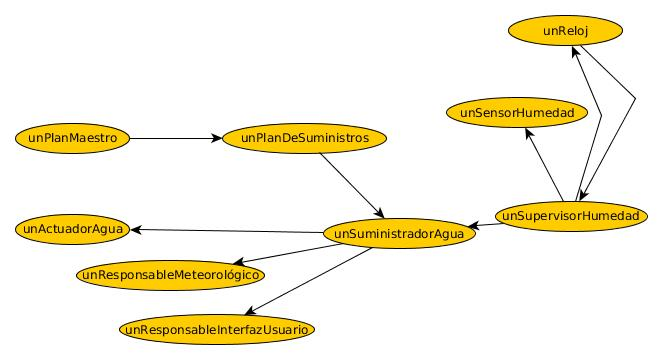
\includegraphics[width=0.6\textwidth]{./imagenes/objetosCoordinador.jpg}
  \caption{Diagrama de colaboración de objetos}
  \label{fig:sec_sum1}
\end{figure}

\begin{figure}[h!]
  \centering
  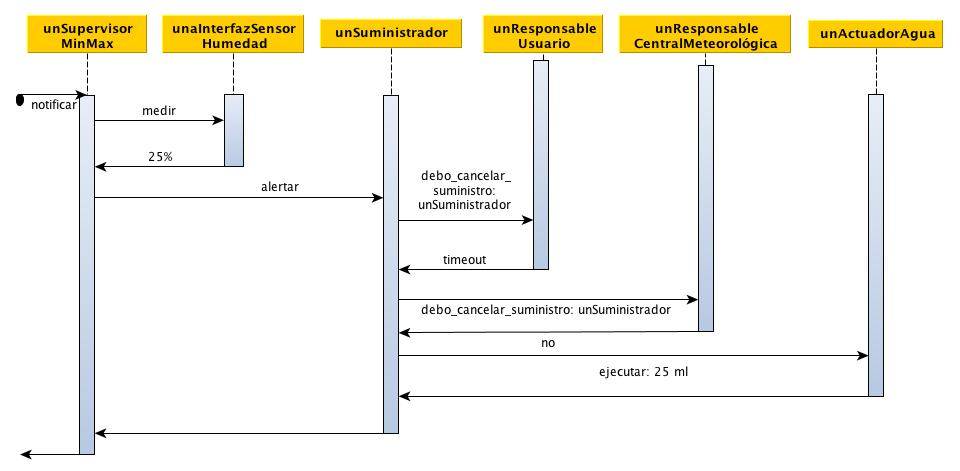
\includegraphics[width=0.8\textwidth]{./imagenes/secuencia_suministro1.jpg}
  \caption{Diagrama de secuencia de regulación realizada}
  \label{fig:sec_sum1}
\end{figure}

\clearpage

\begin{figure}[h!]
  \centering
  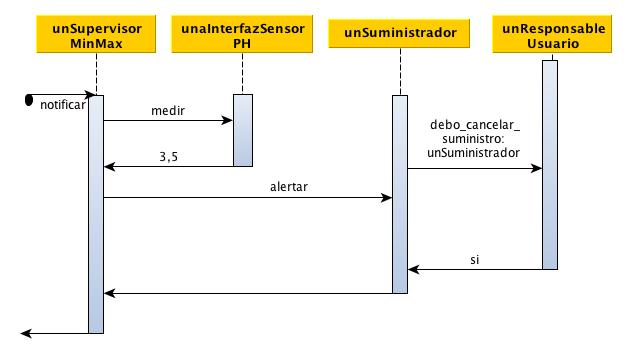
\includegraphics[width=0.6\textwidth]{./imagenes/secuencia_suministro2.jpg}
  \caption{Diagrama de secuencia de regulación abortada}
  \label{fig:sec_sum1}
\end{figure}

\begin{figure}[h!]
  \centering
  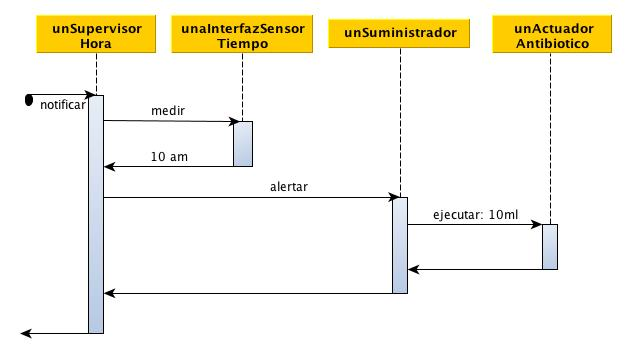
\includegraphics[width=0.6\textwidth]{./imagenes/secuencia_suministro3.jpg}
  \caption{Diagrama de secuencia de suministro programado}
  \label{fig:sec_sum1}
\end{figure}

\section{Conclusiones}
Como resumen de las conclusiones vertidas a lo largo del informe podemos mencionar las siguientes:

La implementación de Scrum exclusivamente entre programadores inexpertos en el uso de la metodología termina recayendo en una suerte de "waterfall" con deadlines cortos, debido a la metodologías a las que venimos acostumbrados. Posiblemente sea más eficiente mezclar programadores expertos con inexpertos para una mayor eficiencia en la implementación.

Descubrimos que el diseño de un sistema, incluso los más simples, se van mejorando paso a paso, comprendiendo más profundamente el significado de las palabras "iterativo-incremental". También descubrimos la inmensa utilidad de la comunicación con el "product owner".
